

\documentclass[11pt,a4paper]{article}
\usepackage{lac2017}
\usepackage[utf8]{inputenc}
\usepackage{graphicx}
\usepackage{balance}
\usepackage{ifpdf}
\usepackage{hyperref}
\usepackage{amssymb,amsmath} 
\usepackage{verbatim}
\usepackage{color}
%\usepackage[small,labelfont=bf, indention=1cm]{caption}
\usepackage[small,labelfont=bf,hang,indention=-1cm,justification=raggedright]{caption}

\sloppy
\newenvironment{contentsmall}{\small}

\definecolor{mygrey}{gray}{0.95}
\definecolor{captiongrey}{gray}{0.3}
\definecolor{labelcolor}{rgb}{0.5, 0.2, 0.2}

\captionsetup{labelfont={color=labelcolor,bf},textfont={color=captiongrey}} 

\newcommand{\OSC}[1]	{{\fontsize{10pt}{10pt} \selectfont\texttt{#1}}}
\newcommand{\tab}		{\hspace*{4mm}}
\newcommand{\dtab}		{\tab \tab}

\newcommand{\sample}[1]	{\vspace{-0.2em}\begin{center}\colorbox{mygrey}{\begin{minipage}[t]{0.98\columnwidth} {\small \texttt{#1}}\end{minipage}}\end{center}}



\title{Towards dynamic and animated music notation using INScore}

%see lac2015.sty for how to format multiple authors!
\author
{Dominique Fober, Yann Orlarey \and Stéphane Letz
\\ GRAME - Centre national de création musicale 
\\ 11 cours de Verdun Gensoul
\\ 69002 Lyon
\\ France, 
\\ \{fober, orlarey, letz\}@grame.fr 
}



\begin{document}
\maketitle


\begin{abstract}
\begin{contentsmall}
INScore is an environment for the design of augmented interactive music scores opened to conventional and non-conventional use of the music notation. The system has been presented at LAC 2012 and has significantly evolved since, with improvements turned to dynamic and animated notation. This paper presents the latest features and notably the dynamic time model, the events system, the scripting language, the symbolic scores composition engine, the network and Web extensions, the interaction processes representation system and the set of sensor objects.
\end{contentsmall}
\end{abstract}

\keywords{
\begin{contentsmall}
INScore, music score, dynamic score, interaction.
\end{contentsmall}
}

%------------------------------------------------------
\section{Introduction}

Contemporary music creation poses numerous challenges to the music notation. Spatialized music, new instruments, gesture based interactions, real-time and interactive scores, are among the new domains that are now commonly explored by the artists. 
Common music notation doesn't cover the needs of these new musical forms and numerous research and approaches have recently emerged, testifying to the maturity of the music notation domain, in the light of computer tools for music notation and representation.
Issues like writing spatialized music \cite{Ellberger_tenor2015}, addressing new instruments \cite{tmays:2014} or new interfaces \cite{kschlei:2015} (to cite just a few), are now subject of active research and proposals.

Interactive music and real-time scores are also representative of an expanding domain in the music creation field. The advent of the digital score and the maturation of the computer tools for music notation and representation constitute the basement for the development of this musical form, which is often grounded on non-traditional music representation \cite{RSmith_tenor2015} \cite{Hope_tenor2015} but may also use the common music notation \cite{Hoadley12,hoadley14}. 

In order to address the notation challenges mentioned above, INScore \cite{Fober:10c} has been designed as an environment opened to non-conventional music representation (although it supports symbolic notation), and turned to real-time and interactive use \cite{Fober:13b}. It is clearly focused on music representation only and in this way, differs from tools integrated into programming environments like Bach \cite{agostini12b} or MaxScore \cite{didko08}. 

INScore has been already presented at LAC 2012 \cite{Fober:12a}. It has significantly evolved since and this paper introduces the set of issues that have been more recently addressed. After a brief recall of the system and of the programming environment, we'll present the scripting language extensions and the symbolic scores composition engine that provides high level operations to describe real-time and interactive symbolic scores composition. Next we'll describe how interaction processes representations can be integrated into the music score and how remote access is supported using the network and/or Web extensions. Tablet and smartphone support have led to integrate gestural interaction with a set of \emph{sensor} objects that will be presented. Finally, the time model, recently extended, will be described.


%------------------------------------------------------
\section{The INScore environment}
INScore is an environment to design interactive augmented music scores. It extends the music representation to arbitrary graphic objects (symbolic notation but also images, text, vectorial graphics, video, signals representation) and provides an homogeneous approach to manipulate the score components both in the graphic and time spaces. 

It supports \emph{time synchronization in the graphic space}, which refers to the graphic representation of the temporal relations between components of a score - via a synchronization mechanism and using \emph{mappings} that express relations between time and graphic space segmentations (Fig. \ref{fig:sync}).
\begin{figure}[ht]
\begin{center}
	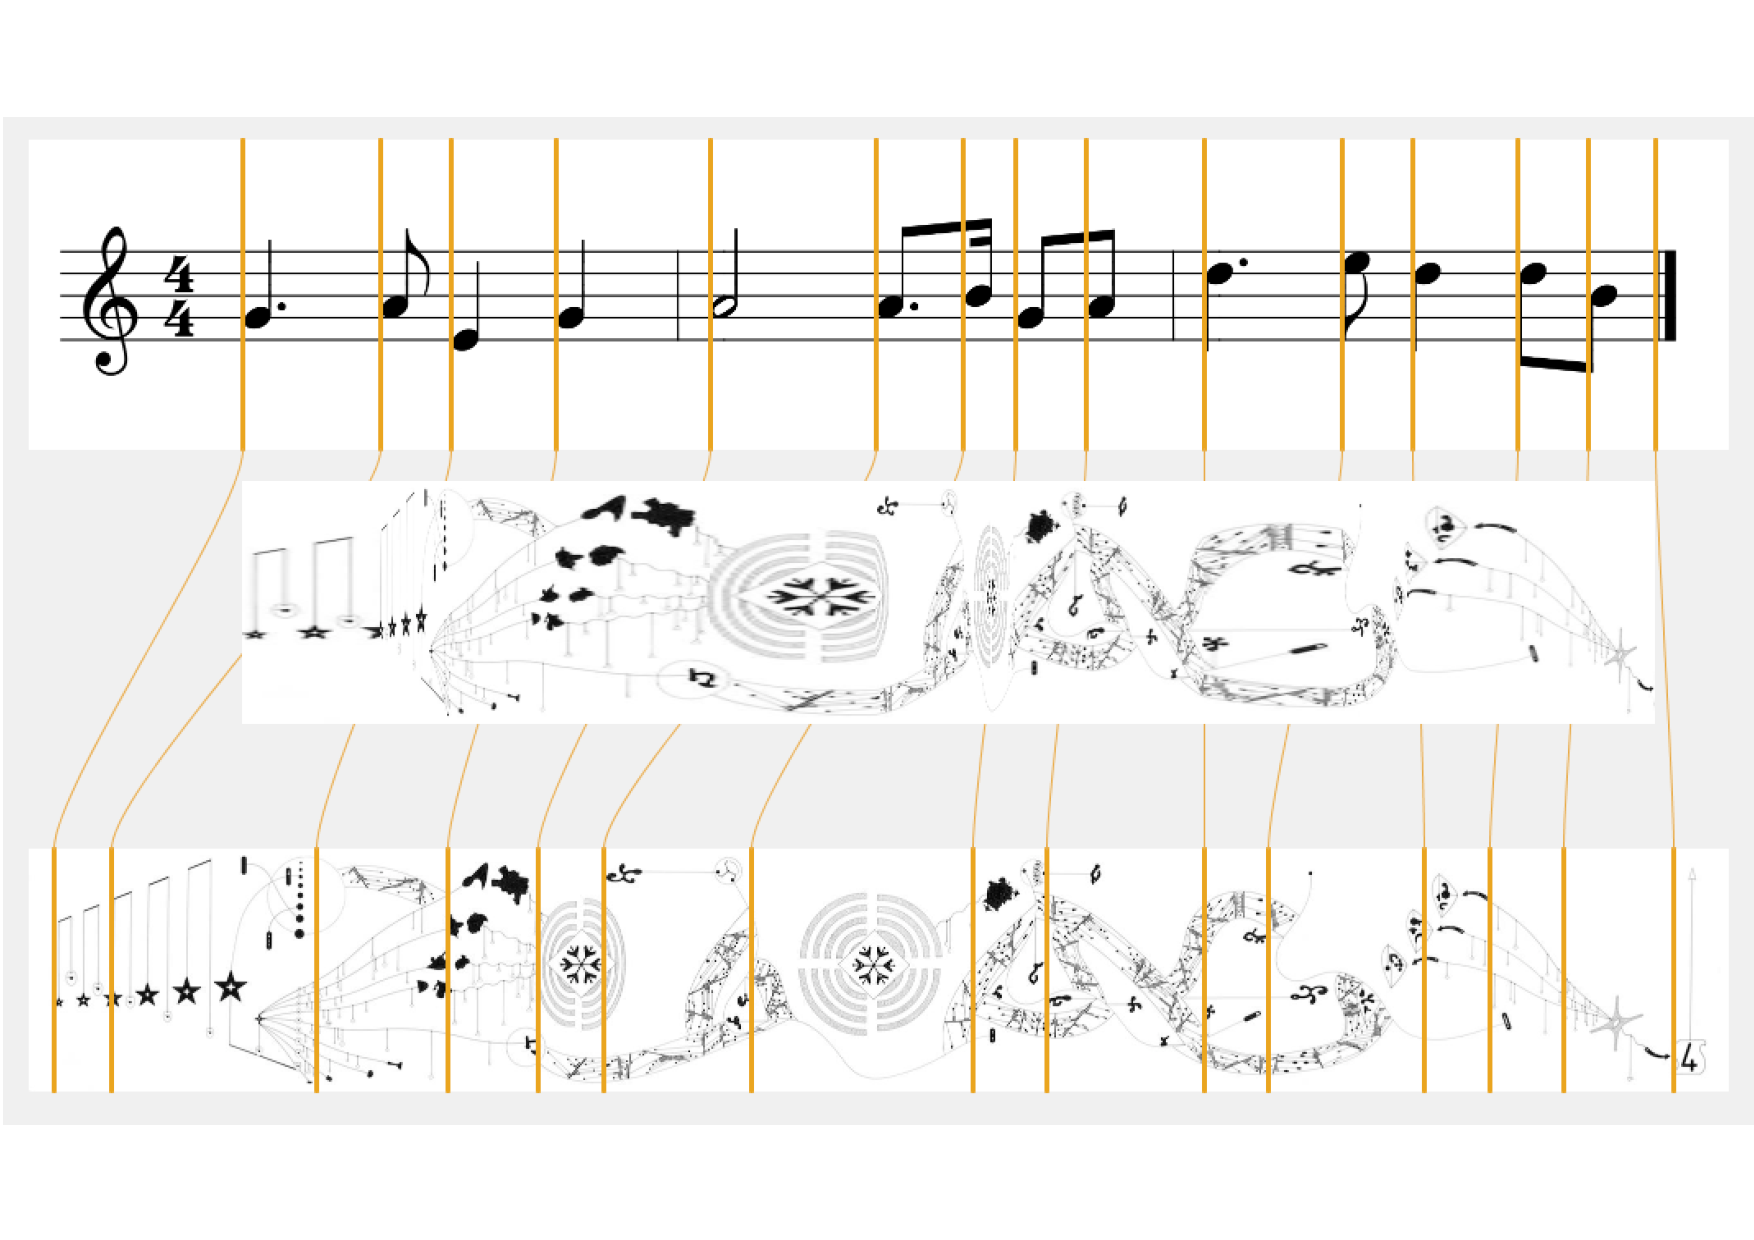
\includegraphics[width=1.\columnwidth]{imgs/syncAB}
\caption{A graphic score (Mark Applebaum's graphic score \emph{Metaphysics of Notation}) is synchronized to a symbolic score. The picture in the middle is the result of the synchronization. The vertical lines express the graphic to graphic relationship, that have been computed by composing the objects common relations with the time space.}
\label{fig:sync}
\end{center}
\end{figure}

INScore has been primarily designed to be controlled via OSC\footnote{\url{http://opensoundcontrol.org/}} messages. The format of the messages consists in an OSC address followed by a message string and 0 to n parameters (Fig. \ref{fig:osc}). 
\begin{figure}[ht]
\begin{center}
	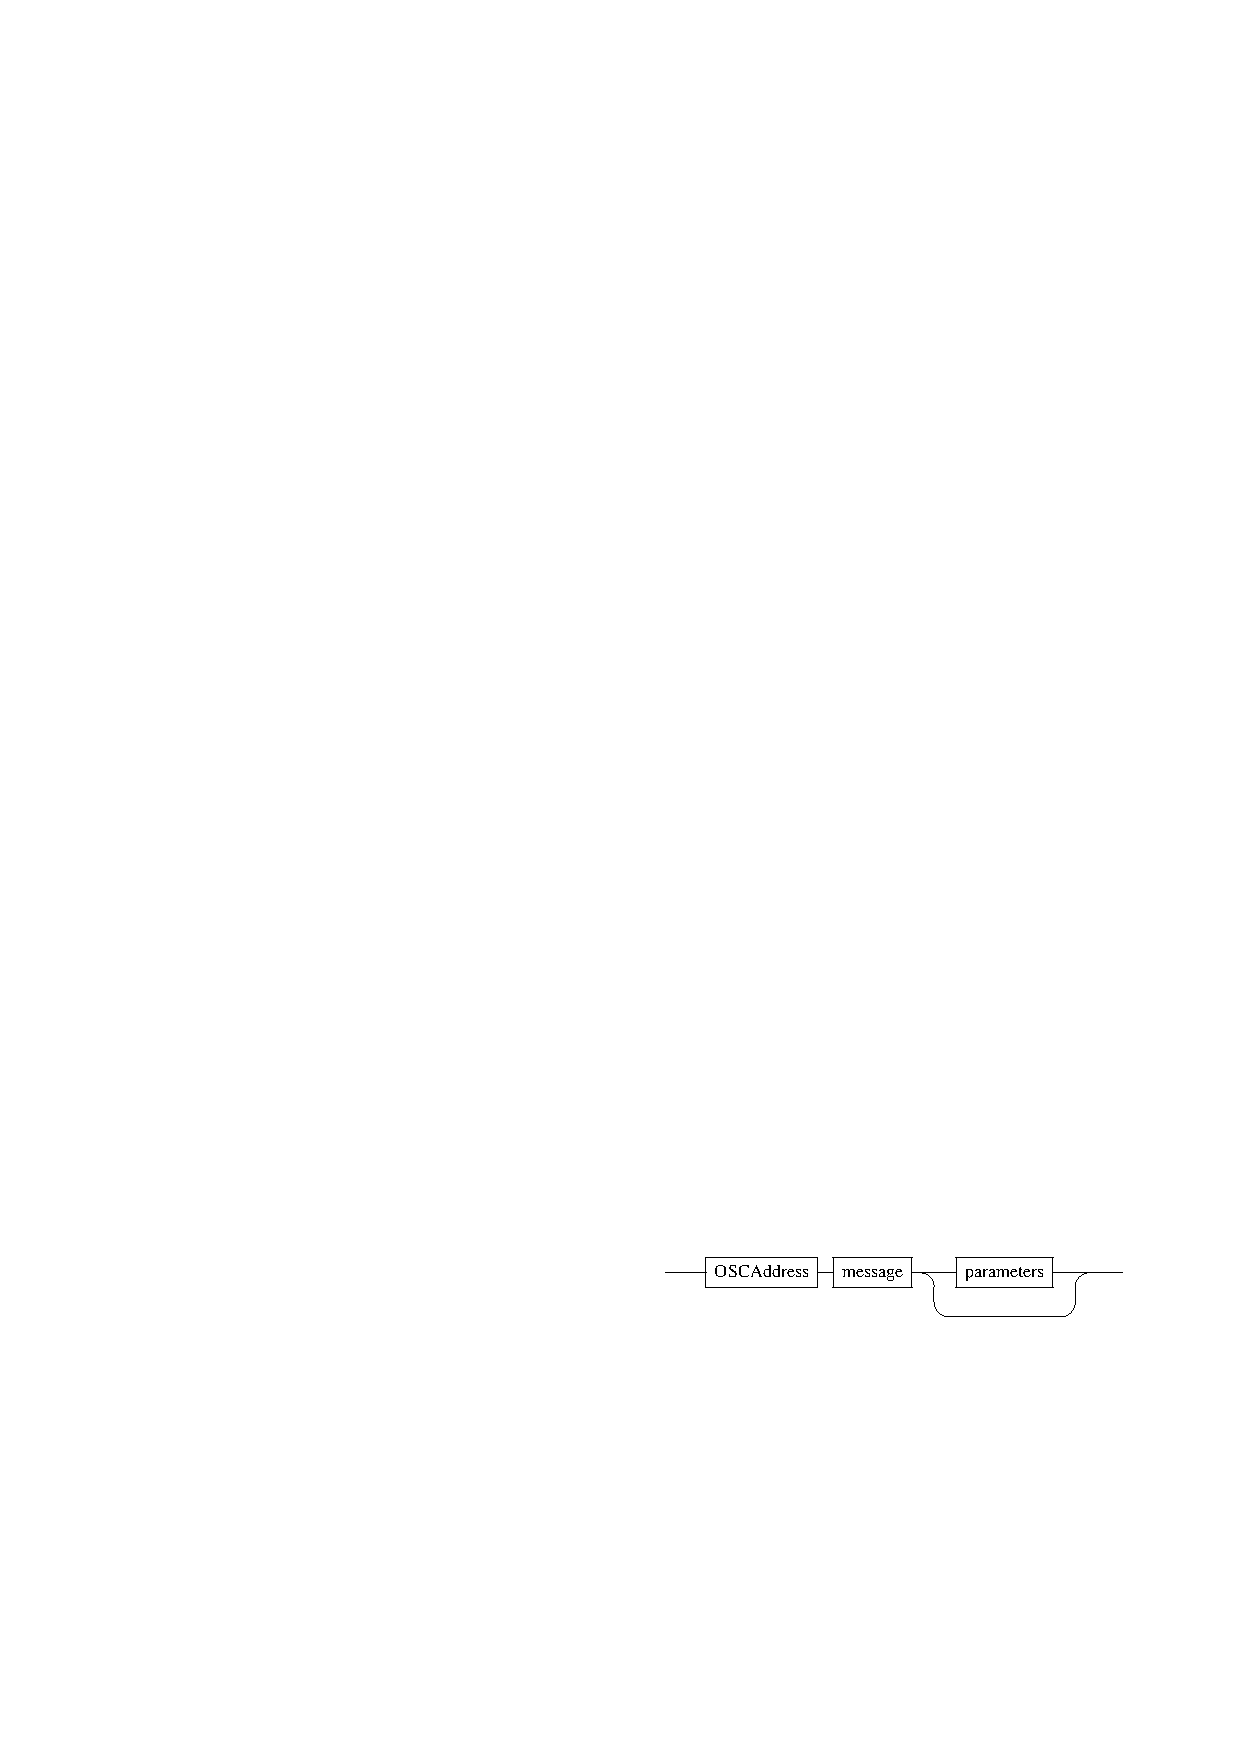
\includegraphics[width=1.\columnwidth]{imgs/oscformat}
\caption{INScore messages general format.}
\label{fig:osc}
\end{center}
\end{figure}

Compared to object oriented programming, the address may be viewed as an object pointer, the message string as a method name and the parameters as the method parameters. For example, the message:\\
\tab \OSC{/ITL/scene/score color 255 128 40 150} \\
may be viewed as the following method call: \\
\tab \OSC{ITL[scene[score]]->color(255 128 40 150)}

The system provides a set of messages for the graphic space control (\OSC{x, y, color, space,} etc.), for the time space control (\OSC{date, duration,} etc.), and to manage the environment. It includes two special messages:
\begin{itemize}
\item the \OSC{set} message that operates like a constructor and that takes the object type as parameter, followed by type specific parameters (Fig. \ref{fig:set}).
\item the \OSC{get} message provided to query the system state  (Fig. \ref{fig:get}).
\end{itemize}

%--------------------------
\begin{figure}[ht]
\begin{center}
\sample{/ITL/scene/obj set txt "Hello world!";
}
\caption{A message that creates a textual object, which type is \OSC{txt}, with a text as specific data.}
\label{fig:set}
\end{center}
\end{figure}

%--------------------------
\begin{figure}[ht]
\begin{center}
\sample{/ITL/scene/obj get;\\
\tab -> /ITL/scene/obj set txt "Hello world!";\\
\\
/ITL/scene/obj get x y;\\
\tab -> /ITL/scene/obj x 0;\\
\tab -> /ITL/scene/obj y 0.5;
}
\caption{Querying an object with a \OSC{get} message gives messages on output (prefixed with \OSC{->}). These messages can be used to restore the corresponding object state.}
\label{fig:get}
\end{center}
\end{figure}

The address space is dynamic and not limited in depth. It is hierarchically organized, the first level \OSC{/ITL} is used to address the application, the second one 
\OSC{/ITL/\textit{scene}} 
to address the score and the next ones to address the components of a score (note that \textit{scene} is a default name that can be user defined). Arbitrary hierarchy of objects is supported.

%------------------------------------------------------
\section{The scripting language}
The OSC messages described above have been turned into a textual version to constitue the INScore scripting language. This language has been rapidly extended to support :
\begin{itemize}
\item variables, that may be used to share parameters between messages (Fig. \ref{fig:var}).
\item message based variables and/or parameters that consists in querying an object to retrieve one of it's attributes value (Fig. \ref{fig:msgvar}).
\item an extended OSC addressing scheme that allows to send OSC messages to an external application for initialization of control purposes (Fig. \ref{fig:eosc}).
\item JavaScript sections that can be evaluated at parsing and/or run time. A JavaScript call is expected to produce INScore messages as output (Fig. \ref{fig:java}).
\item mathematical expressions (\OSC{+ - / *, conditionals}, etc.) that can be used for arguments computation (Fig. \ref{fig:math}).
\item symbolic scores composition expressions that are described in section \ref{sec:scorecompo}. 
\end{itemize}

%--------------------------
\begin{figure}[ht]
\begin{center}
\sample{greylevel = 140;\\
color = \$greylevel \$greylevel \$greylevel; \\
/ITL/scene/obj1 color \$color; \\
/ITL/scene/obj2 color \$color;
}
\caption{Variables may be used to share values between messages.}
\label{fig:var}
\end{center}
\end{figure}

%--------------------------
\begin{figure}[ht]
\begin{center}
\sample{ox = \$(/ITL/scene/obj get x);\\
/ITL/scene/obj2 x \$(/ITL/scene/obj get x);
}
\caption{The output of \OSC{get} messages can be used by variables or as another message parameter.}
\label{fig:msgvar}
\end{center}
\end{figure}

%--------------------------
\begin{figure}[ht]
\begin{center}
\sample{/ITL/scene/obj set txt "Hello world!"; \\
localhost:8000/start;
}
\caption{This script initialises a textual object and sends the \OSC{/start} message to an external application listening on UDP port 8000.}
\label{fig:eosc}
\end{center}
\end{figure}

%--------------------------
\begin{figure}[ht]
\begin{center}
\sample{<?javascript \\
\tab function randpos(address) \{\\
\tab \tab var x = (Math.random() * 2) - 1;\\
\tab \tab return address + " x " + x + ";"; \\
\tab\}\\
?> \\
/ITL/scene/javascript run \\
\tab \tab \tab \tab 'randpos("/ITL/scene/obj")'; 
}
\caption{The JavaScript section defines a \OSC{randpos} function that computes an \OSC{x} message with a random value, addressed to the object given as parameter. This function may be next called at initialization or at any time using the static JavaScript node embedded into each score.}
\label{fig:java}
\end{center}
\end{figure}

%--------------------------
\begin{figure}[ht]
\begin{center}
\sample{/ITL/scene/o x (\$shift ? \$x + 0.5 : \$x);
}
\caption{A mathematical expression is used to compute the position of an object depending on 2 previously defined variables. }
\label{fig:math}
\end{center}
\end{figure}
 

%------------------------------------------------------
\section{Symbolic scores composition}
\label{sec:scorecompo}

Rendering of symbolic music notation makes use of the Guido engine \cite{Dau:09b}. Thus the primary music score description format is the Guido Music Notation format \cite{hoos98} [GMN]. The MusicXML format \cite{good01} is also supported via conversion to the GMN format. 

The Guido engine provides a set of operators for scores level composition \cite{fober12b}. These operators consistently take 2 scores as argument to produce a new score as output. They allow to put scores in sequence \OSC{(seq)}, in parallel \OSC{(par)}, to cut a score in the time dimension \OSC{(head, tail)}, in the polyphonic dimension \OSC{(top, bottom)}, to transpose \OSC{(transpose)}, to stretch \OSC{(duration)} a score and to apply the rhythm or the pitch of a score to another one \OSC{(rhythm, pitch)}.

The INScore scripting language includes \emph{score expressions}, a simple language providing score composition operations. 
The novelty of the proposed approach relies on the dynamic aspects of the operations, as well as on the persistence of the score expressions. A score may be composed as an arbitrary graph of score expressions and equipped with a fine control over the changes propagation.

%----------------------------------
\subsection{Score expressions}

A score expression is defined as an operator followed by two scores (Fig. \ref{fig:scexpr}). The leading \OSC{expr} token is present to disambiguate parenthesis in the context of INScore scripts.
\begin{figure}[ht]
\begin{center}
	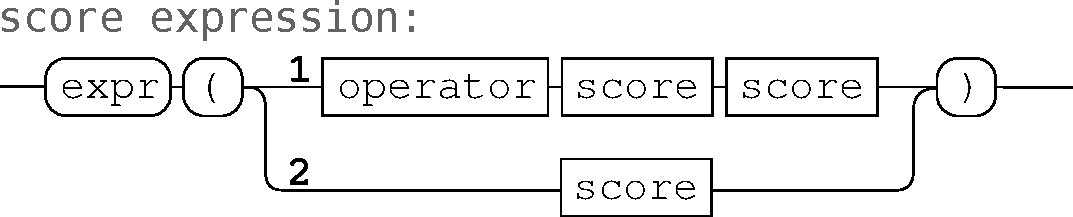
\includegraphics[width=1.\columnwidth]{imgs/score-expr}
\caption{Score expressions syntax.}
\label{fig:scexpr}
\end{center}
\end{figure}

The score arguments may be:
\begin{itemize}
\item a literal score description string (GMN or MusicXML formats),
\item a file (GMN or MusicXML formats),
\item an existing score object,
\item a score expression.
\end{itemize}
An example is presented in Fig. \ref{fig:scex1}.
%--------------------------
\begin{figure}[ht]
\begin{center}
\sample{expr( par score.gmn (seq "[c]" score))
}
\caption{A score expression that puts a score file (\OSC{score.gmn}) in parallel with the sequence of a literal score and an existing object (\OSC{score}). Note that the leading \OSC{expr} token can be omitted inside an expression.}
\label{fig:scex1}
\end{center}
\end{figure}

%----------------------------------
\subsection{Dynamic score expression trees}

The score expressions language is first transformed into an internal tree representation. In a second step, this representation is evaluated to produce GMN strings as output, that are finally passed to the INScore object as specific data. 

Basically, the tree is reduced using a depth first post-order traversal and the result is stored in a cache. However, the score expressions language provides a mechanism to make arbitrary parts of a tree variable using an ampersand (\&) as prefix of an argument, preventing the corresponding nodes to be reduced at cache level (Fig. \ref{fig:scex2}). 
    
\begin{figure}[ht]
\begin{center}
\sample{expr( par score.gmn (seq "[c]" \&score))
}
\caption{A score expression that includes a reference to a \OSC{score} object. Successive evaluations of the expression may produce different results, provided that the \OSC{score} object has changed.}
\label{fig:scex2}
\end{center}
\end{figure}

INScore events system (described in section \ref{events}) provides a way to automatically trigger the re-evaluation of an expression when one  of it's variable parts has changed. These mechanisms open the door to dynamic scores composition within the INScore environment.
More details about the score expressions language can be found in \cite{Lepetit-Aimon_tenor2016}.


%----------------------------------
\section{Musical processes representation}

INScore includes tools for the representation of musical processes within the music score. In the context of interactive music and/or when a computer is involved in a music performance, it may provide useful information regarding the state of the musical processes running on the computer. This feedback can notably be used to guide the interaction choices of the performer.

On INScore side, a process state is viewed as a signal. Signals are part of a score components and can be combined into \emph{graphic signals} to become first order objects of a score. They may be notably used for the representation of a performance \cite{Fober:12a}. 

Regarding musical processes representation, a signal can be connected to any attribute of an object (Fig. \ref{fig:sig}), which makes the signal variations visible (and thus the process activity) with the changes of the corresponding attributes.

%--------------------------
\begin{figure}[ht]
\begin{center}
\sample{/ITL/scene/signal/sig size 100; \\
/ITL/scene/obj set rect 0.5 0.5; \\
/ITL/scene/img set img 'file.png'; \\
/ITL/scene/signal connect sig \\
\dtab"obj:scale" "img:rotatez[0,360]";
}
\caption{A signal \OSC{sig} is connected to the \OSC{scale} attribute of an object and to the \OSC{rotatez} attribute of an image. Note that for the latter, the signal values (expected to be in [-1,1]) are scaled to the interval [0,360].}
\label{fig:sig}
\end{center}
\end{figure}

%----------------------------------
\section{Network and Web dimensions}

INScore supports the aggregation of distributed resources over Internet, as well as the publication of a score via the HTTP and/or WebSocket protocols. In addition, a score can also be used to control a set of remote scores on the local network using a \emph{forwarding} mechanism.


%----------------------------------------
\subsection{Distributed score components}

Most of the components of a score can be defined in a literal way or using a file. All the file based resources can be specified as a simple file path, using absolute or relative path, or as an HTTP url (Fig \ref{fig:files}). 

%--------------------------
\begin{figure}[ht]
\begin{center}
\sample{/ITL/scene/obj1 set img 'file.png';\\
/ITL/scene/obj2 set img \\
\dtab \tab 'http://www.adomain.org/file.png';
}
\caption{File based resources can refer to local or to remote files.}
\label{fig:files}
\end{center}
\end{figure}

When using a relative path, an absolute path is built using the current path of the score, that may be set to an arbitrary location using the \OSC{rootPath} attribute of the score (Fig \ref{fig:rootpath}). 

%--------------------------
\begin{figure}[ht]
\begin{center}
\sample{/ITL/scene rootPath '/users/me/inscore';\\
/ITL/scene/obj set img 'file.png';;
}
\caption{The \OSC{rootPath} of a score is equivalent to the current directory in a shell. With this example, the system will look for the file at '/users/me/inscore/file.png'}
\label{fig:rootpath}
\end{center}
\end{figure}

The current rootpath can also be set to an arbitrary HTTP url, so that further use of a relative path will result in an url (Fig. \ref{fig:rooturl}).

%--------------------------
\begin{figure}[ht]
\begin{center}
\sample{/ITL/scene rootPath \\
\dtab \dtab \dtab 'http://www.adomain.org';\\
/ITL/scene/obj set img 'file.png';;
}
\caption{The \OSC{rootPath} supports urls. With this example, the system will look for the file at 'http://www.adomain.org/file.png'}
\label{fig:rooturl}
\end{center}
\end{figure}

This mechanism allows to mix local and remote resources in the same music score, but also to express local and remote scores in a similar way, just using a \OSC{rootPath} change.


%----------------------------------------
\subsection{HTTPd and WebSocket objects}

A music score can be published on the Internet using the HTTP or the WebSocket protocols. Specific objects can be embedded in a score in order to make this score available to remote clients (Fig. \ref{fig:servers}).

%--------------------------
\begin{figure}[ht]
\begin{center}
\sample{/ITL/scene/http set httpd 8000; \\
  /ITL/scene/ws set websocket 8100 200;
}
\caption{This example creates an httpd server listening on the port 8000 and a WebSocket server listening on the port 8100 with a  maximum notification rate of 200 ms.}
\label{fig:servers}
\end{center}
\end{figure}

The WebSocket server allows bi-directional communication between the server and the client. It sends notifications of score changes each time the graphic appearance of the score is modified, provided that the notification rate is lower than the maximum rate set at server creation time. 

The communication scheme between a client and an INScore Web server relies on a reduced set of messages. These messages are protocol independent and are equally supported over HTTP or WebSocket :
\begin{itemize}
\item \OSC{get}: requests an image of the score.
\item \OSC{version}: requests the current version of the score. The server answers with an integer value that is increased each time the score is modified.
\item \OSC{post}: intended to send an INScore script to the server.  
\item \OSC{click}: intended to allow remote mouse interaction with the score.
\end{itemize}

More details are available from \cite{Fober:15b}.


%----------------------------------------
\subsection{Messages forwarding}\label{forward}

Message forwarding is another mechanism provided to distribute scores over a network. It operates at application and/or score levels when the \OSC{forward} the message is send to the application (\OSC{/ITL}) or to a score (\OSC{/ITL/scene}). 
The message takes a list of destination hosts specified using a host name or an IP number, and suffixed with a port number. All the OSC messages may be forwarded, provided they are not filtered out (Fig. \ref{fig:forward}).
The filtering strategy is based on OSC adresses and/or on INScore methods (i.e. messages addressing specific objects attributes). 
%--------------------------
\begin{figure}[h]
\begin{center}
\sample{/ITL forward 192.168.1.255:7000; \\
/ITL/filter reject \\
\dtab'/ITL/scene/javascript';
}
\caption{The application is requested to forward all messages on INScore port (7000) to the local network using a broadcast address. Messages addressed to the JavaScript engine are filtered out in order to only forward the result of their evaluation.}
\label{fig:forward}
\end{center}
\end{figure}


%----------------------------------
\section{The \emph{sensor} objects}

INScore runs on the major operating systems including Android and iOS. Tablet and smartphone support have led to integrate gestural interaction with a set of sensor (Table \ref{tabsensors}). 

Sensors can be viewed as objects or as signals. When created as a signal node, a sensor behaves like any signal but may provide some additional features (like calibration). When created as a score element, a sensor has no graphical appearance but provides specific sensor events and features.

\begin{table}[ht]
\begin{center}
\begin{tabular}{rl}
\hline
name & values \\
\hline
accelerometer	& x, y, z \\
ambient light	& light level \\
compass			& azimuth \\
gyroscope		& x, y, z \\
light			& a level in lux \\
magnetometer	& x, y, z \\
orientation		& device orientation \\
proximity		& a boolean value \\
rotation		& x, y, z \\
tilt			& x, y \\
\hline
\end{tabular}
\end{center}
\caption{The set of sensors and associated values}
\label{tabsensors}
\end{table}

All the sensors won't likely be available on a given device. In case a sensor is not supported, an error message is generated at creation request and the creation process fails.



%----------------------------------
\section{The time model}

INScore time model has been recently extended to support \emph{dynamic} time. Indeed and with the initial design, the time attributes of an object are fixed and don't change unless a time message \OSC{(date, duration)} is received, which can only be emitted from an external application or using the \emph{events} mechanism. The latter (defined very early) introduced another notion of time: the \emph{events} time, which takes place when an event occurs.  The \emph{events} system has also been extended for more flexibility. 

%----------------------------------
\subsection{The musical time}
Regarding the time domain, any object of a score has a date and a duration. A new tempo attribute has been added, which has the effect of moving the object in the time dimension when non null, according to the tempo value and the absolute time flow. 
Let $t_0$ be the time of the last tempo change of an object, let $v$ be the tempo value, the object date $d_t$ at a time $t$ is given by a time function $f$:
\begin{equation}
%\[
	 f(t) \to d_t = d_t{_0} + (t - t_0) \times v \times k , \quad t \geqq t_0
%\]
\label{timeeq}
\end{equation}
where $d_i$ is the object date at time $t_i$ and $k$ a constant to convert absolute time in musical time.
In fact, absolute time is expressed in milliseconds and the musical time unit is the whole note. Therefore, the value of $k$ is $1 / 1000 \times 60 \times 4$.

Each object of a score has an independent tempo. The tempo value is a signed integer, which means that an object can move forward in time but backward as well.

From implementation viewpoint and when its tempo is not null, an object sends \OSC{ddate} (a relative displacement in time) to itself at periodic intervals (Fig. \ref{fig:tempo}).

\begin{figure}[h]
   \centering
   \sample{/ITL/scene/obj tempo 60 \\
   \\
-> /ITL/scene/obj ddate $f(r_i)$ \\
-> /ITL/scene/obj ddate $f(r_{i+1})$ \\
-> /ITL/scene/obj ddate $f(r_{i+2})$ \\
-> ...
}
   \caption{A sequence of messages that activate the time of an object \OSC{obj}. Messages prefixed by \OSC{->} are generated by the object itself. $r_{i}$ is the value of the absolute time elapsed between the task $i$ and $i-1$.}
   \label{fig:tempo}
\end{figure}

This design is consistent with the overall system design since it is entirely message based. It is thus compatible with all the INScore mechanisms such as the forwarding system.


%----------------------------------
\subsection{The events system}
\label{events}

The event-driven approach of time in INScore preceded the musical time model and has been presented in \cite{Fober:13b}. 
The event-based interaction process relies on messages that are associated to events and that are sent when the corresponding event occurs. The general format of an interaction message is described in Fig. \ref{fig:watch}.

\begin{figure}[ht]
\centerline{
	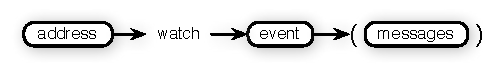
\includegraphics[width=0.95\columnwidth]{imgs/watch}}
\caption{Format of an interaction message: the \OSC{watch} request installs a messages list associated to the event \OSC{event}.}
\label{fig:watch}
\end{figure}

Initially, the events typology was limited to classical user interface events (e.g. mouse events), extended in the time domain (see Table~\ref{tbl:evts}). 

\begin{table}[htp]
\begin{center}
\begin{tabular}{c|c}
Graphic domain & Time domain \\
\hline
mouseDown 		& timeEnter	\\
mouseUp			& timeLeave	\\
mouseEnter		& durEnter		\\
mouseLeave		& durLeave		\\
mouseMove		&				\\
\end{tabular}
\end{center}
\caption{Main INScore events in the initial versions.}
\label{tbl:evts}
\end{table}%

This typology has been significantly extended to include:
\begin{itemize}
\item touch events \OSC{(touchBegin, touchEnd, touchUpdate)}, available on touch screens and supporting multi-touch.
\item any attribute of an object: modifying an object attribute may trigger the corresponding event, that carries the name of the attribute (e.g. \OSC{x, y date}, etc.). 
\item an object specific data i.e. defined with a \OSC{set} message. The event name is \OSC{newData} and has been introduced for the purpose of the symbolic score composition system.
\item user defined events, that have to comply to a special naming scheme.
\end{itemize}
\vspace*{1mm}
Any event can be triggered using the \OSC{event} message, followed by the event name and event's dependent parameters. The \OSC{event} message may be viewed as a function call that generates OSC messages on output. This approach is particularly consistent for user events that can take an arbitrary number of parameters, which are next available to the associated messages under the form of variables named  $\$1...\$n$ (Fig. \ref{fig:uevent}).


\begin{figure}[h]
   \centering
   \sample{/ITL/scene/obj watch MYEVENT ( \\
\tab/ITL/scene/t1 set txt \$1, \\
\tab/ITL/scene/t2 set txt \$2 \\
);   \\   
/ITL/scene/obj event MYEVENT \\
\hspace*{25mm}"This text is for t1"\\
\hspace*{25mm}"This one is for t2"; 
}
   \caption{Definition of a user event named \OSC{MYEVENT} that expects 2 arguments referenced as \$1 and \$2 in the body of the definition. This event is next triggered with 2 different strings as arguments.}
   \label{fig:uevent}
\end{figure}

The time dimension of the events system allows to put \emph{functions} in the time space under the form of events that trigger messages that can modify the score state and/or be addressed to external applications using the extended OSC addressing scheme (Fig. \ref{fig:events}).
  
\begin{figure}[h]
   \centering
   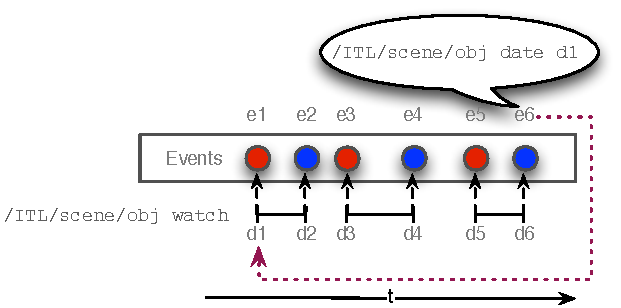
\includegraphics[width=0.95\columnwidth]{imgs/events}
   \caption{Exemple of events placed in the time space. These events are associated to time intervals \OSC{(timeEnter} and \OSC{timeLeave)} and are triggered when entering (in red) of leaving (in blue) these intervals. The last event \OSC{(e6)} emits a  \OSC{date} message that creates a loop by putting the object back at the beginning of the first interval.}
   \label{fig:events}
\end{figure}

Combined with the dynamic musical time, this events system allows to describe autonomous animated score. The example in Fig. \ref{fig:ascore} shows how to describe a cursor that moves forward and backward over a score by watching the time intervals that precedes and follows a symbolic score and by inverting the tempo value. 

\begin{figure}[h]
\begin{center}
   \sample{\# first clear the scene \\
/ITL/scene/* del; \\
\\
\# add a simple symbolic score \\
/ITL/scene/score set gmn '[c d e f g a h c2 ]'; \\
\\
\# add a cursor synchronized to the score \\
/ITL/scene/cursor set ellipse 0.1 0.1;\\
/ITL/scene/cursor color 0 0 250;\\
/ITL/scene/sync cursor score syncTop;\\
\\
\# watch different time zones \\
/ITL/scene/cursor watch timeEnter 2 3 \\
\tab ( /ITL/scene/cursor tempo -60 );\\
\\
/ITL/scene/cursor watch timeEnter -1 0 \\
\tab ( /ITL/scene/cursor tempo 60 );\\
\\
\# and finally start the cursor time \\
/ITL/scene/cursor tempo 60;\\
}
\caption{A cursor that moves forward and backward over a symbolic score.}
\label{fig:ascore}
\end{center}
\end{figure}


%----------------------------------
\section{Conclusion}

INScore\footnote{\url{http://inscore.sf.net})} is an ongoing open source project 
that crystallizes a significant amount of research addressing the problematics of the music notation and representation in regard of the contemporary music creation. It is used in artistic projects and many of the concrete experiences raised new issues that are reflected into some of the system extensions. The domain is quite recent and there are still a lot of open questions that we plan to address in future work and in particular: 
\begin{itemize}
\item turning the scripting language into a \emph{real} programming language would provide a more powerful approach to music score description. The embedded JavaScript engine may already be used for an algorithmic description of a score, but switching from one environment (INScore script) to another one (JavaScript) proved to be a bit tedious.
\item extending the score components to give a time dimension to any of their attributes could open a set of new possibilities, including arbitrary representations of the passage of time.
\end{itemize}
Finally, migrating the INScore native environment to the Web is part of the current plans and should also open new perspectives, notably due to the intrinsic connectivity of Web applications.


\balance
\bibliographystyle{acl}
\bibliography{../interlude}

\end{document}
